\documentclass{beamer}
\usepackage{amsmath}
\usepackage{tikz}
\usepackage{listings}

\title{Rod Cutting Problem}
\author{}
\date{}

\begin{document}

\frame{\titlepage}

\begin{frame}{Problem Statement}
    \textbf{Rod Cutting Problem:}\\
    Given a rod of length $n$ inches and a table of prices $p_i$ for $i = 1, 2, \dots, n$, determine the maximum revenue obtainable by cutting the rod and selling the pieces.

    \vspace{1em}
    \textbf{Example Price Table:}
    \centering
    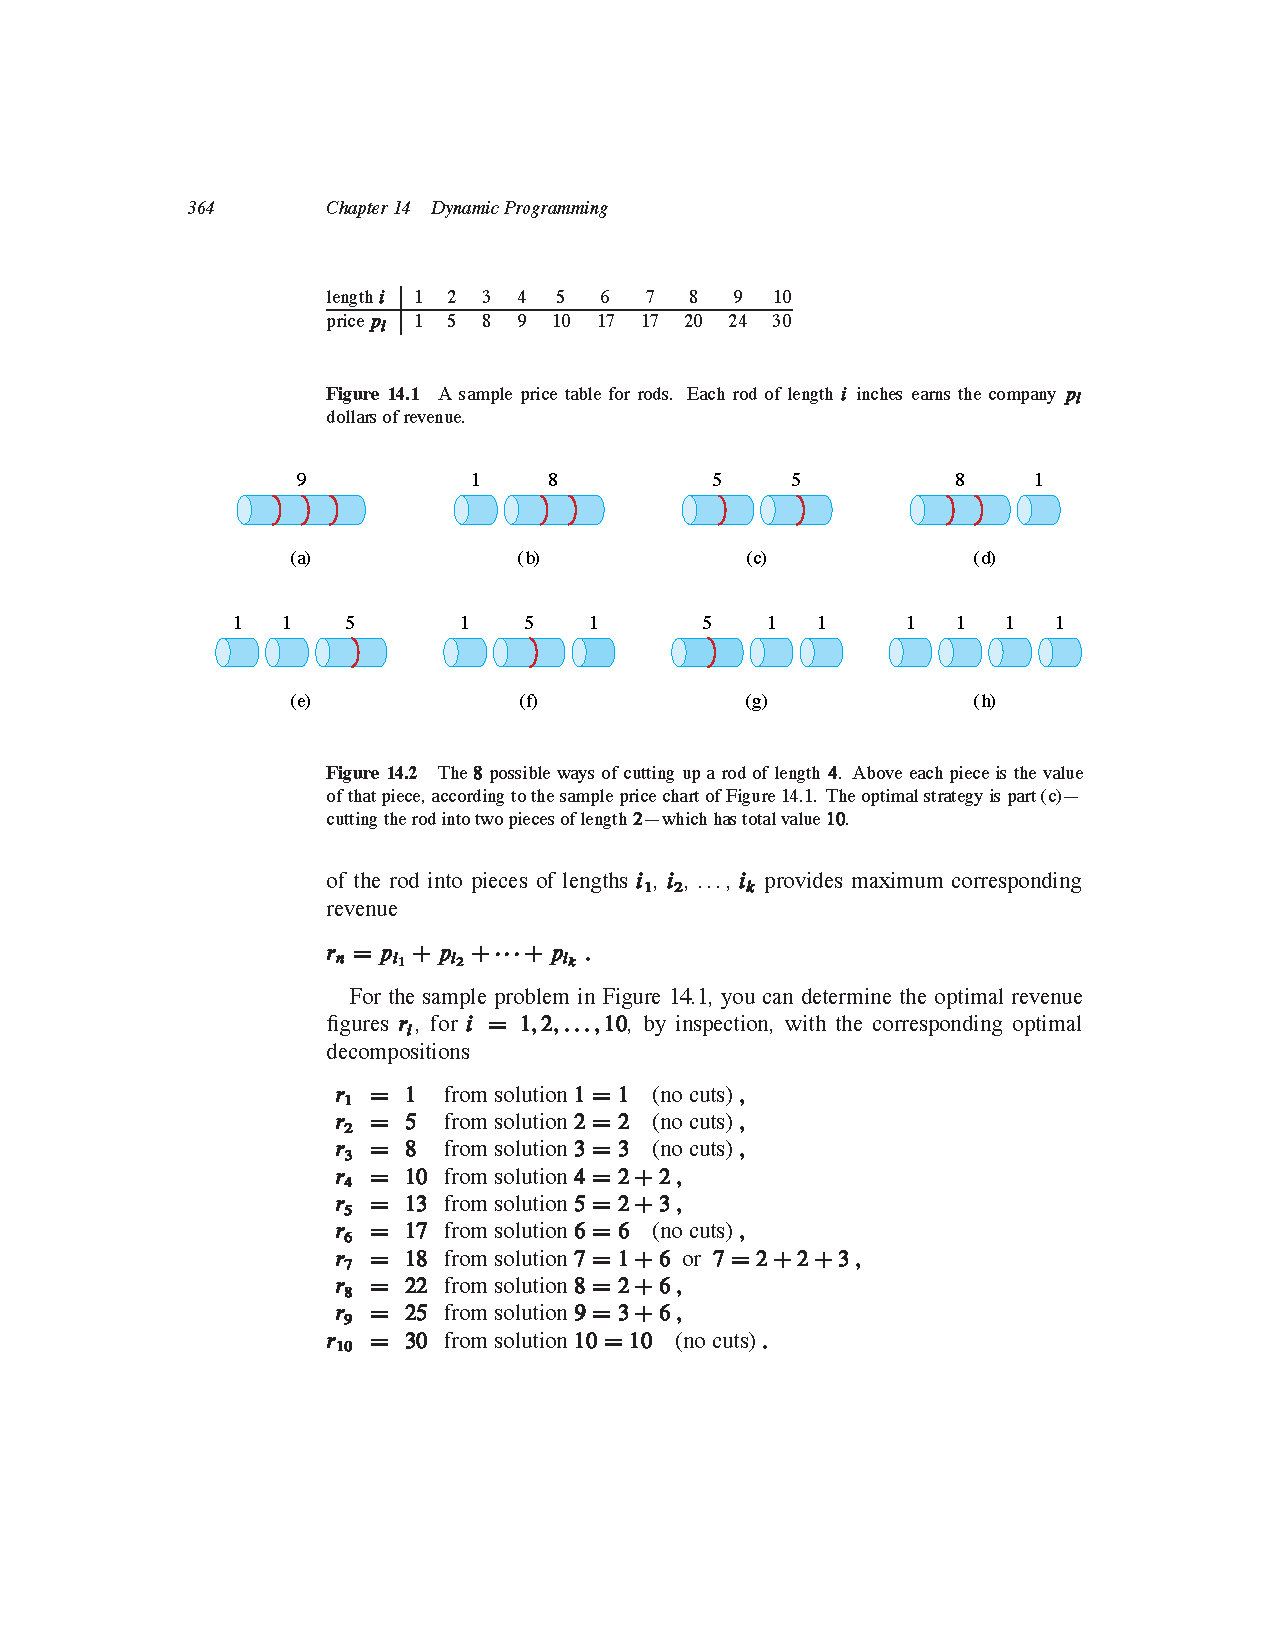
\includegraphics[width=\textwidth,clip=true,trim=5cm 22cm 8cm 4.5cm]{figures/p364}
\end{frame}

\begin{frame}{Problem Statement}
    \centering
    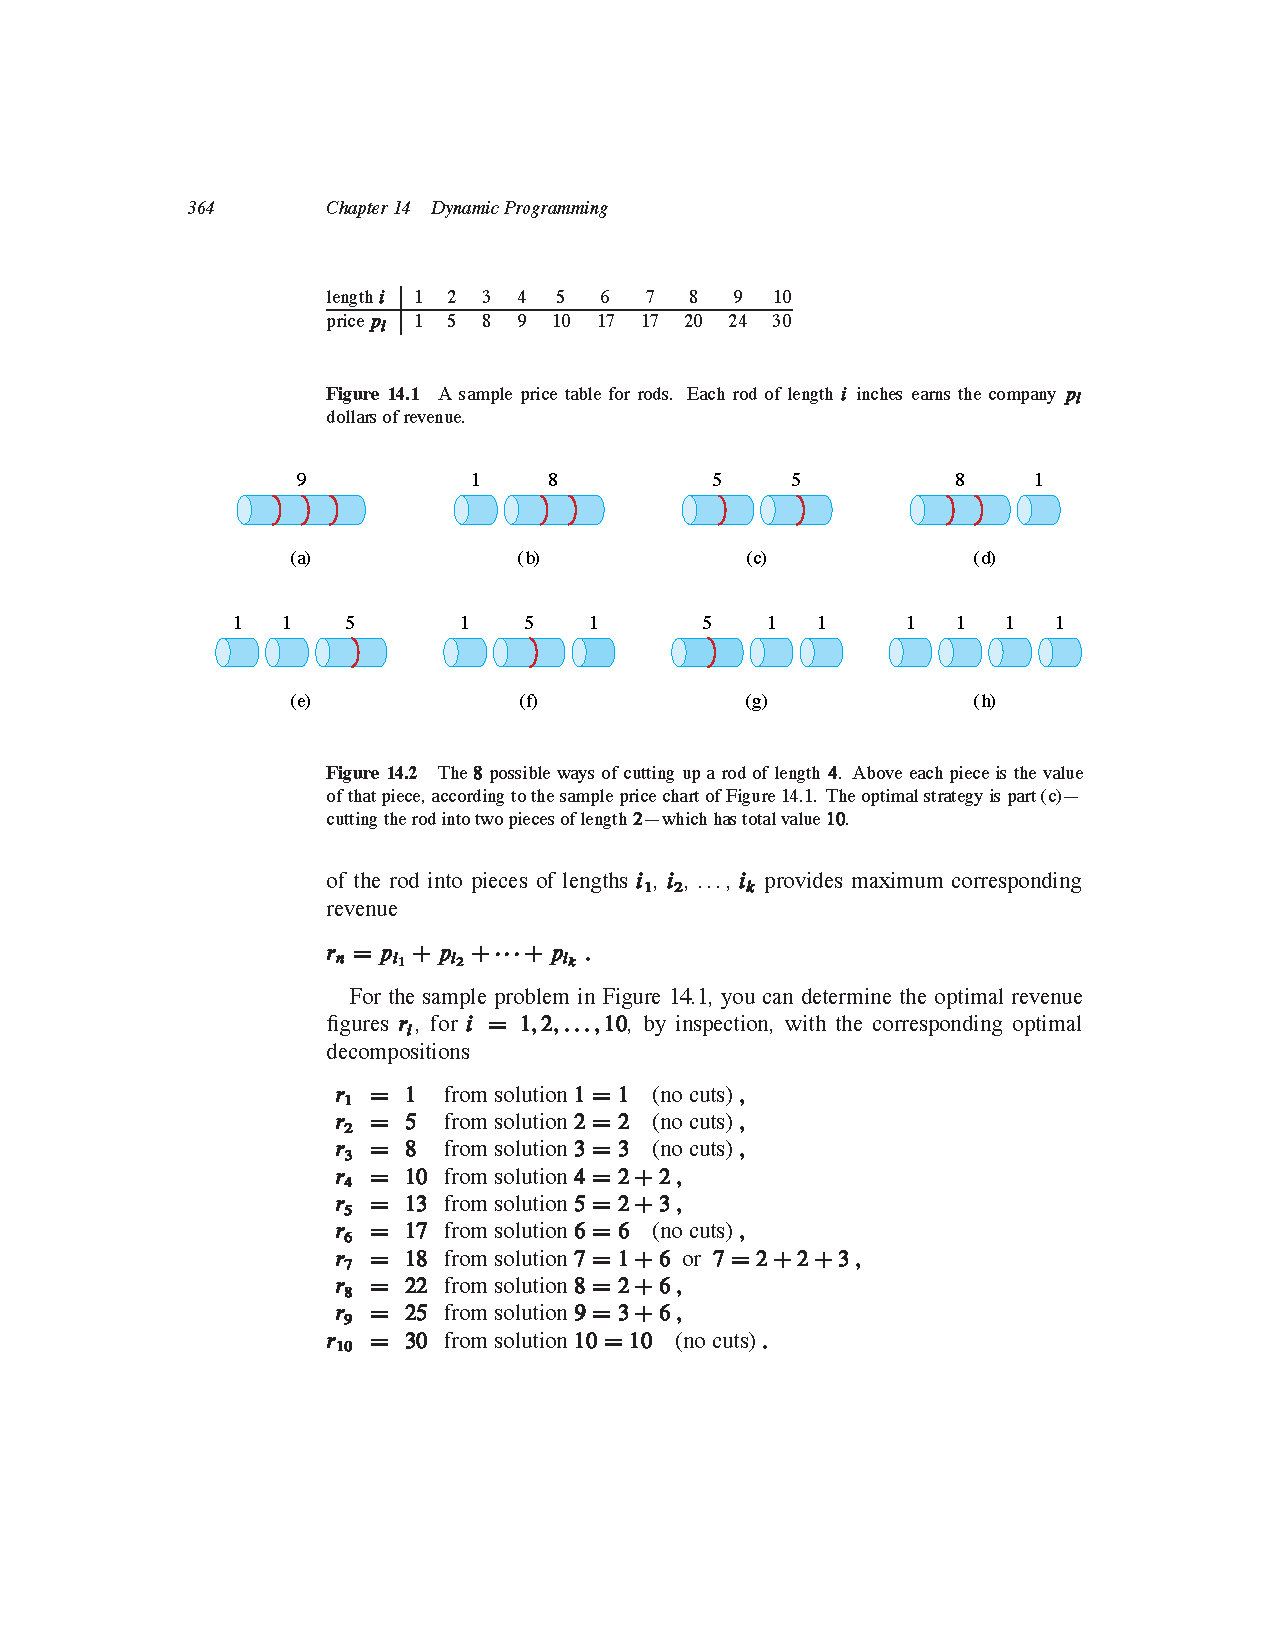
\includegraphics[width=\textwidth,clip=true,trim=3cm 13.5cm 3cm 8cm]{figures/p364}
\end{frame}

\begin{frame}{Recursive Formulation}
    Let $r_n$ be the maximum revenue for a rod of length $n$. Then:

    \[
    r_n = \max_{1 \leq i \leq n} (p_i + r_{n-i})
    \]
    %
    \textbf{Base case:} $r_0 = 0$ \\
    %
    \vspace{1em}
    \textbf{Exponential Time Algorithm:}
    \centering
    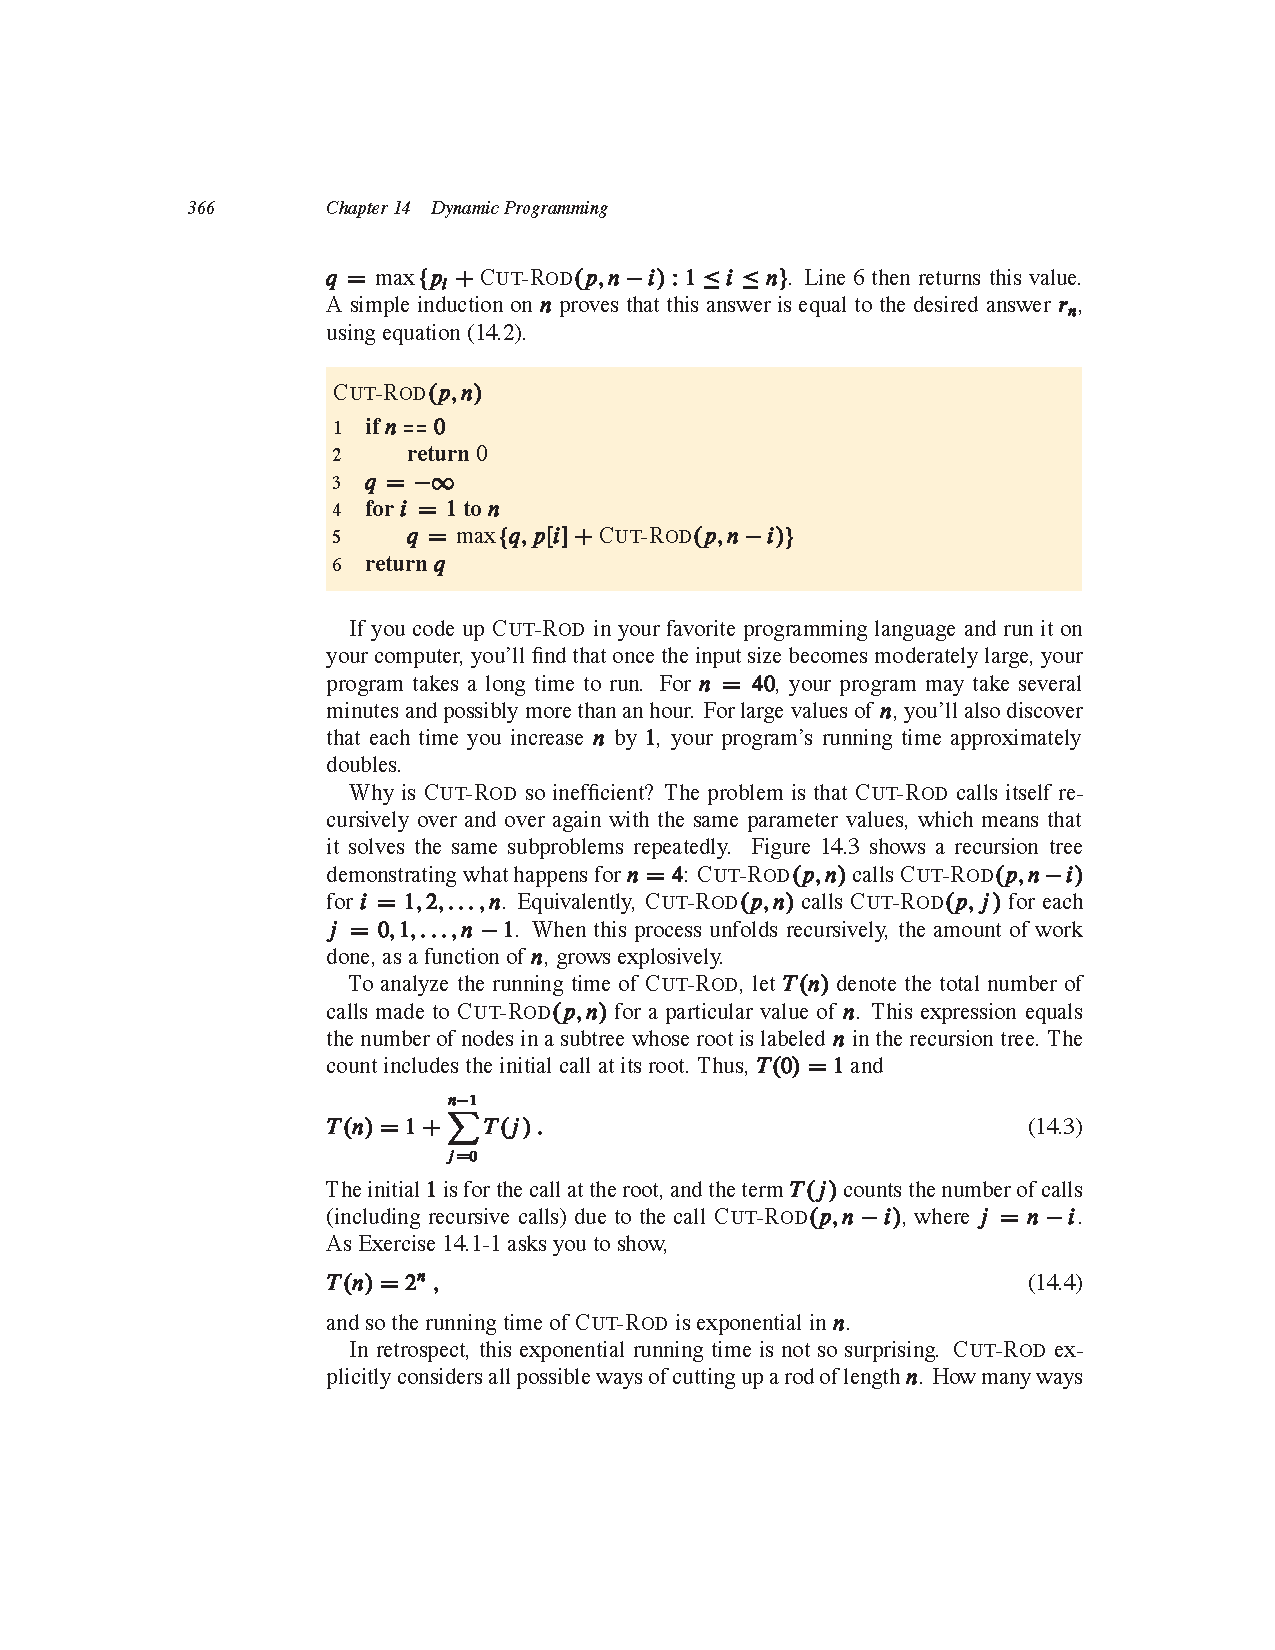
\includegraphics[width=\textwidth,clip=true,trim=4.75cm 18cm 3cm 6cm]{figures/p366}
\end{frame}

\begin{frame}{Recursive Formulation}
    \begin{itemize}
        \item Let $T(n)$ denote the total number of calls made to \textsc{cut-rod}$(p,n)$ for a particular value of $n$.
        \item The number of nodes in a subtree whose root is labeled $n$ in the recursion tree.
    \end{itemize}
    $$
        T(n) = 1 + \sum_{j = 0}^{n - 1} T(j).
    $$
\end{frame}

\begin{frame}{Recursive Formulation}
    \centering
    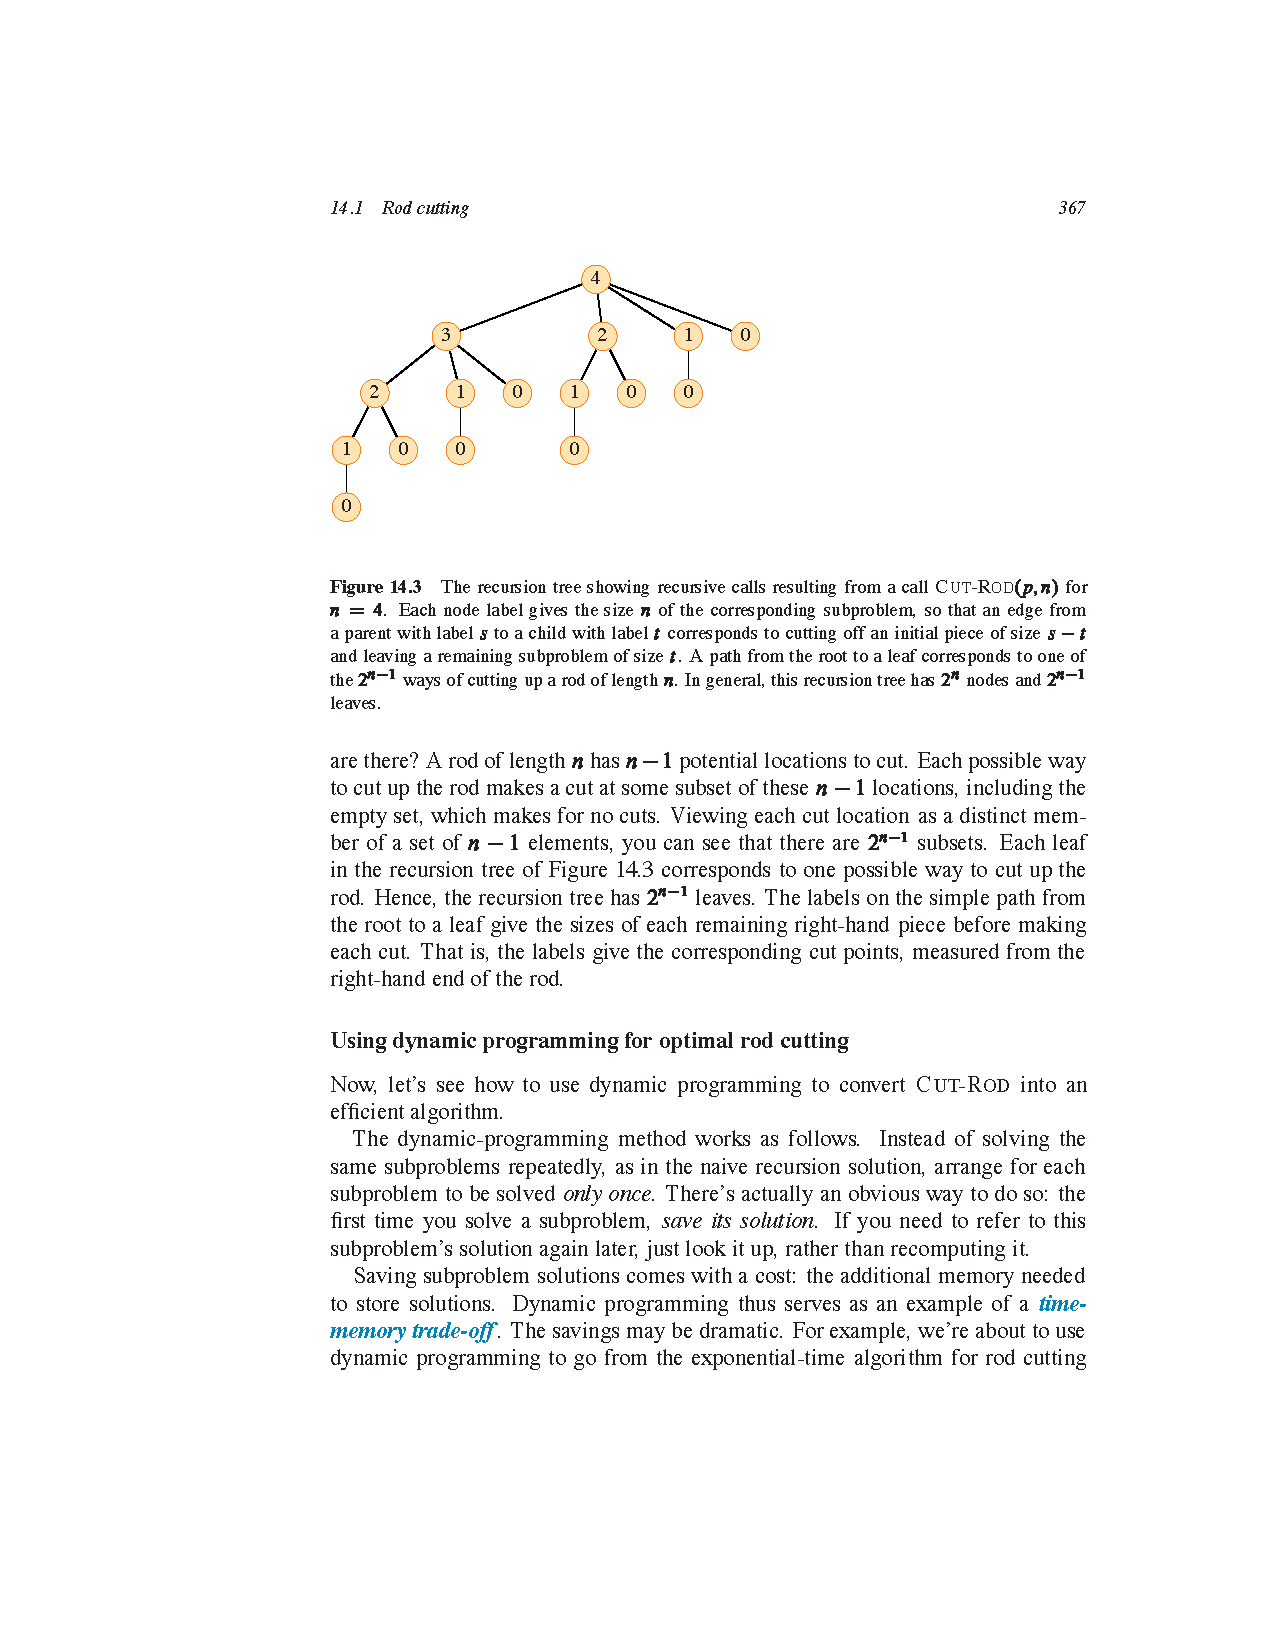
\includegraphics[width=\textwidth,clip=true,trim=5cm 19cm 8cm 4cm]{figures/p367}
\end{frame}

\begin{frame}{Memoized Version}
    Avoids recomputation by storing already computed values.

    \centering
    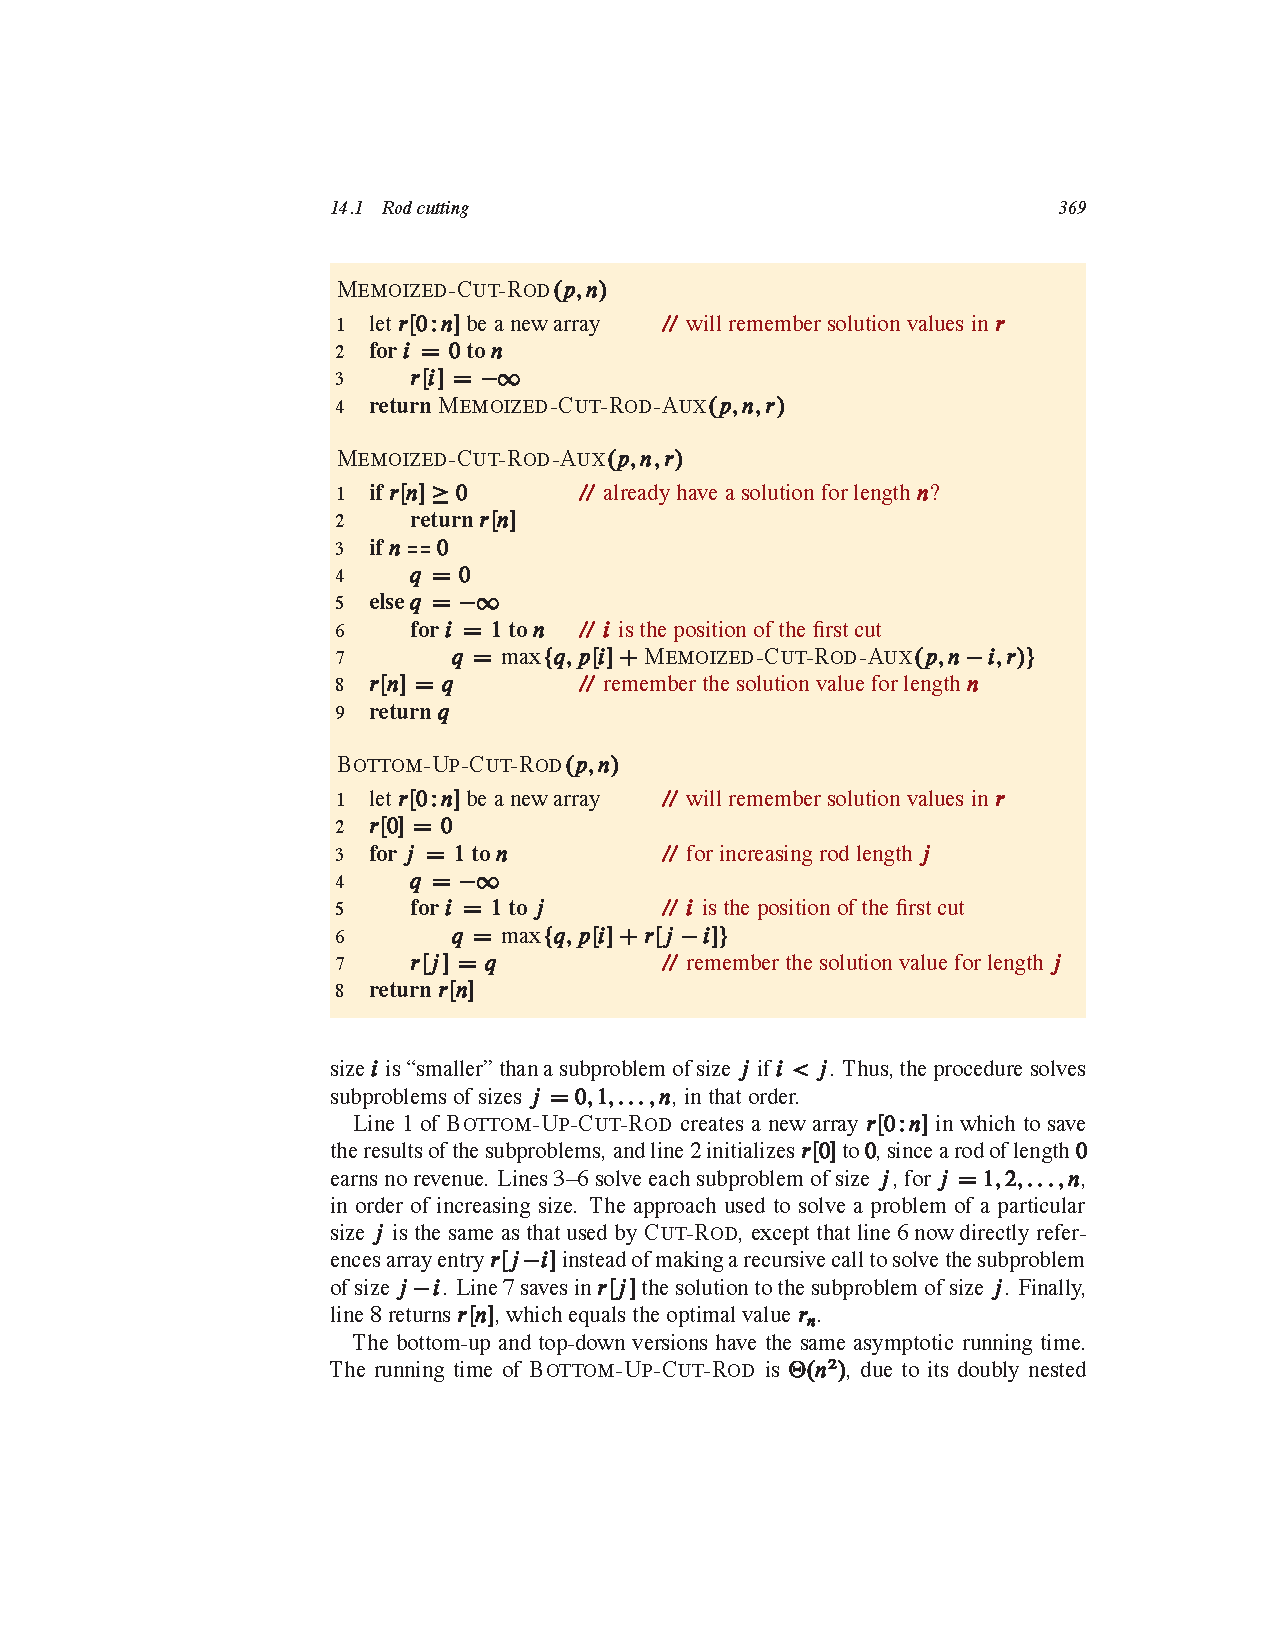
\includegraphics[width=\textwidth,clip=true,trim=5cm 15.5cm 3cm 4cm]{figures/p369}
\end{frame}

\begin{frame}{Bottom-Up Dynamic Programming}
    \centering
    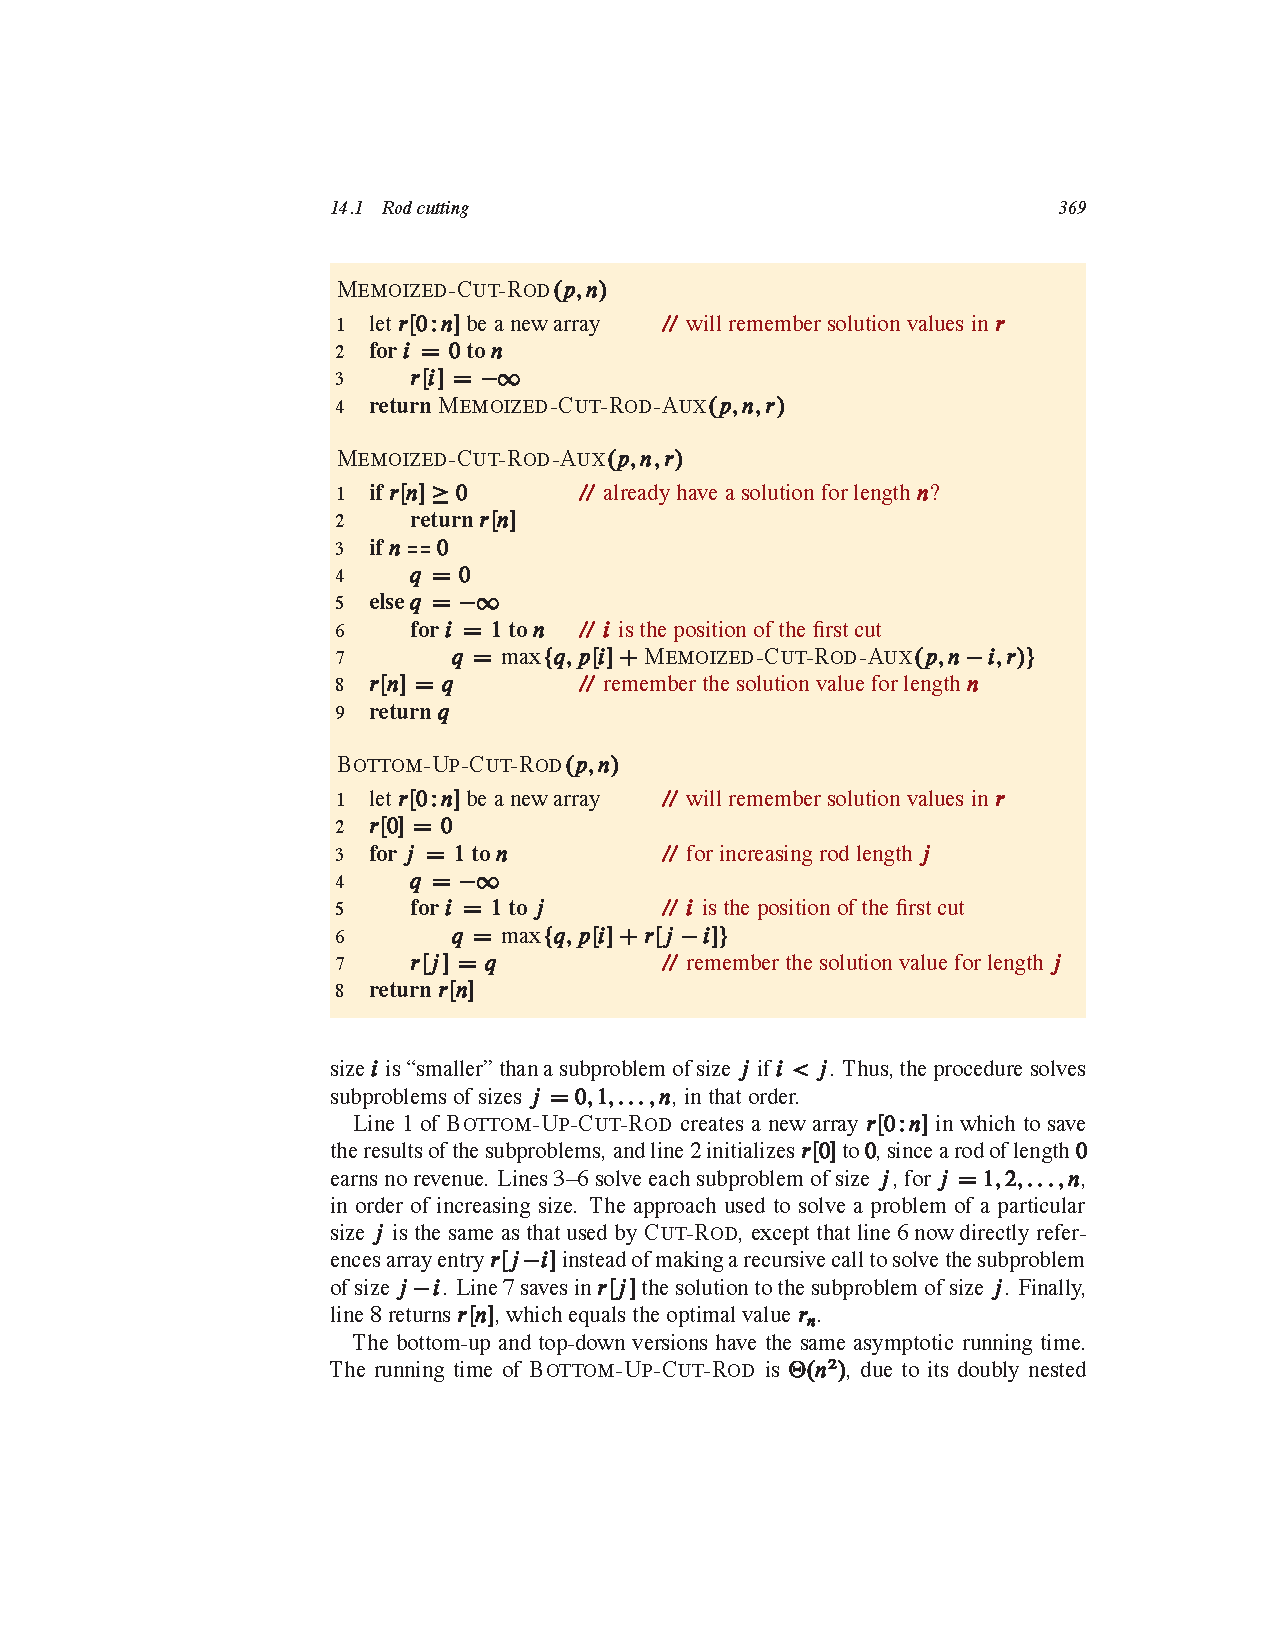
\includegraphics[width=\textwidth,clip=true,trim=5cm 10.5cm 3cm 12.5cm]{figures/p369}

    \textbf{Time complexity:} $\mathcal{O}(n^2)$
\end{frame}

\begin{frame}{Subproblem graphs}
    \centering
    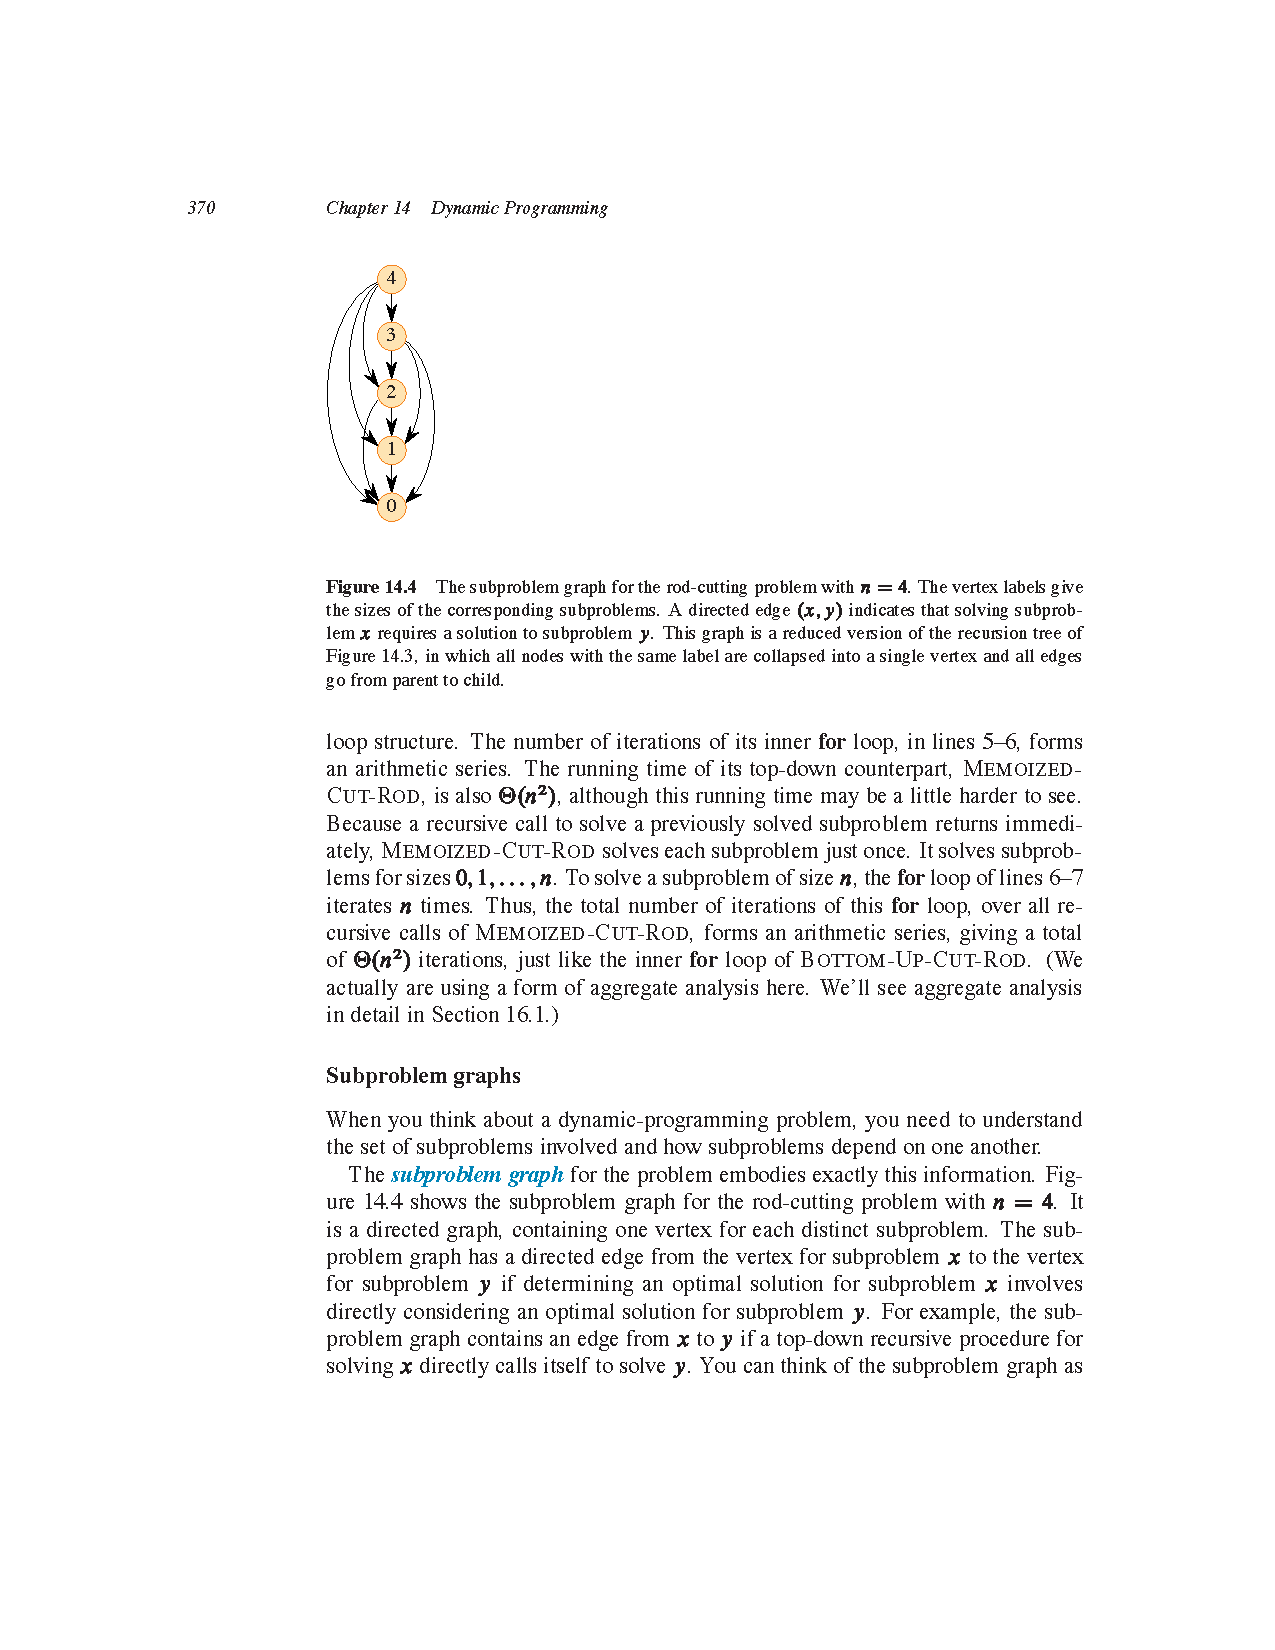
\includegraphics[width=\textwidth,clip=true,trim=5cm 16cm 3cm 4cm]{figures/p370}
\end{frame}

\begin{frame}{Reconstructing the Solution}
    Store the optimal cuts as well:

    \begin{itemize}
        \item Maintain a second array $s[1..n]$.
        \item $s[j]$ stores the length of the first piece to cut from a rod of length $j$.
    \end{itemize}

    Then backtrack using $s[n]$ to print the actual cuts.\\
    \bigskip
    \begin{tabular}{c | r r r r r r r r r r r }
        $i$ & 0 & 1 & 2 & 3 & 4 & 5 & 6 & 7 & 8 & 9 & 10 \\ \hline
        $r[i]$ & 0 & 1 & 5 & 8 & 10 & 13 & 17 & 18 & 22 & 25 & 30 \\
        $s[i]$ &   & 1 & 2 & 3 & 2 & 2 & 6 & 1 & 2 & 3 & 10 \\
    \end{tabular}
\end{frame}

\begin{frame}{Reconstructing a solution}
    \centering
    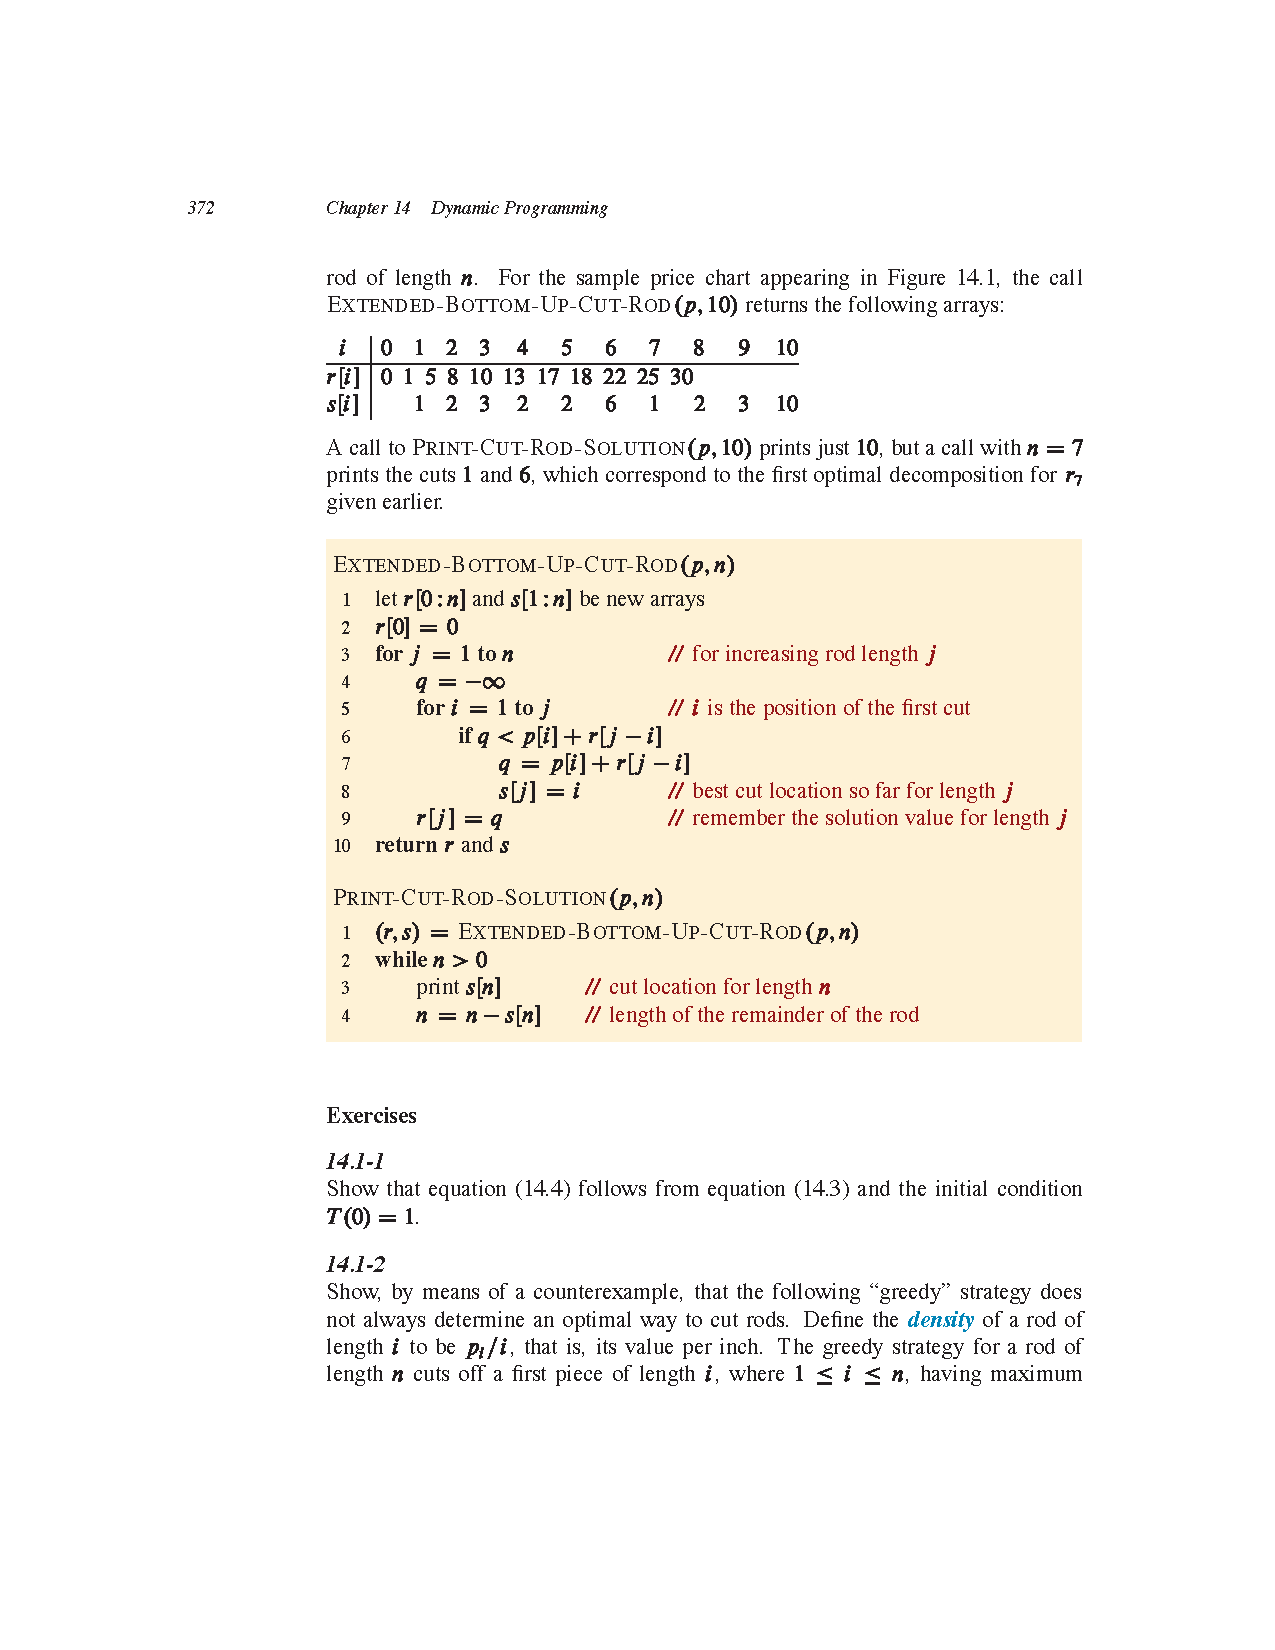
\includegraphics[width=\textwidth,clip=true,trim=5cm 13cm 3cm 9cm]{figures/p372}
\end{frame}

\begin{frame}{Reconstructing a solution}
    \centering
    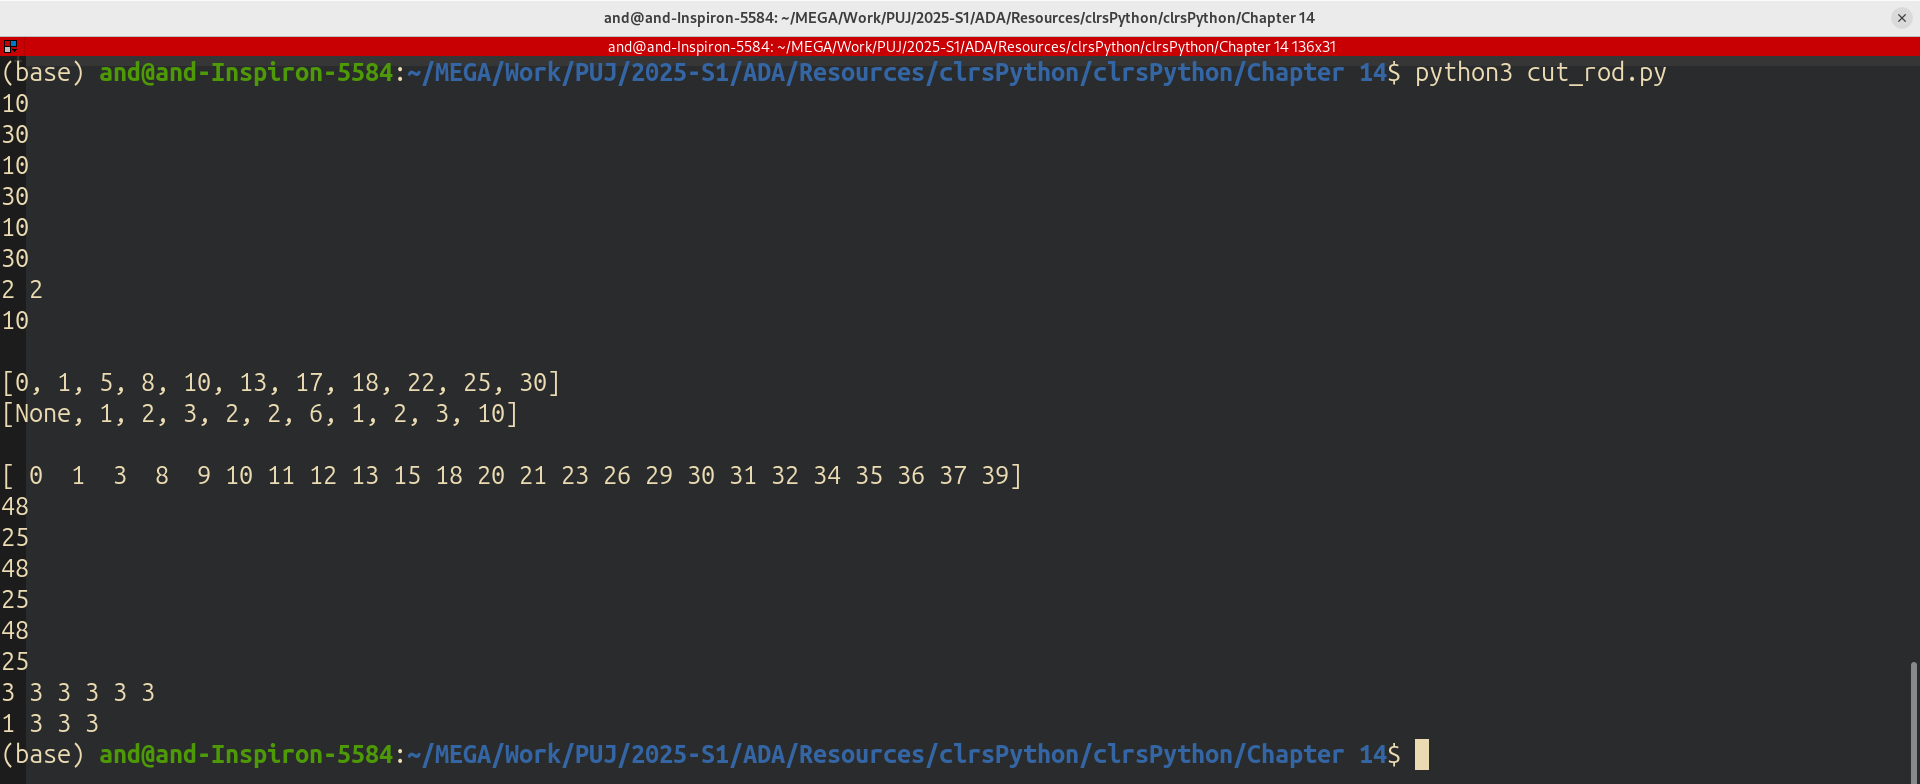
\includegraphics[width=\textwidth]{figures/implementation}
\end{frame}

\begin{frame}{Key Takeaways}
    \begin{itemize}
        \item Naive recursive solution has exponential time complexity
        \item Dynamic programming reduces it to $\mathcal{O}(n^2)$
        \item Optimal substructure and overlapping subproblems make DP suitable
    \end{itemize}
\end{frame}

\end{document}
